\documentclass[conference]{IEEEtran}
\usepackage{cite,amsmath,amssymb,graphicx,algorithm,algpseudocode,booktabs,hyperref}
\usepackage{tikz}
\usetikzlibrary{shapes.geometric,shapes.multipart,arrows.meta,positioning,calc,fit,backgrounds}

\title{A Programmable SumCheck Accelerator for Zero-Knowledge Proofs on FPGA}
\author{Ashesh Kaji\\New York University}

\begin{document}
\maketitle

\begin{abstract}
Zero-Knowledge Proofs (ZKPs) enable privacy-preserving computation but impose severe computational overhead during proof generation. The SumCheck protocol, a core primitive in modern ZKP systems such as HyperPlonk, dominates prover runtime when supporting high-degree custom gates. This work presents an FPGA-based hardware accelerator for a single programmable SumCheck round operating over the BN254 scalar field. The architecture employs eight parallel processing elements, each containing an Extension Engine, Product Lane, Accumulator, and Update Unit, fed by sixteen on-chip scratchpad buffer banks. Modular arithmetic uses the native \texttt{ap\_uint<256>} divider, deferring Montgomery-domain optimization to future work. The design is verified bit-exact against a Python golden model across seven deterministic test cases including multi-term accumulation. Synthesis on a Xilinx RFSoC~4x2 (xczu48dr) at 200~MHz achieves 10.9\% DSP, 7.1\% BRAM, and 30.5\% flip-flop utilization, demonstrating feasibility for integration into a full ZKP prover pipeline.
\end{abstract}

\section{Introduction}

Zero-Knowledge Proofs have emerged as a powerful primitive for secure and privacy-preserving computation, with applications spanning blockchain, machine learning, and verifiable computing~\cite{setty2020spartan}. Despite their promise, ZKPs have seen limited deployment due to exceptionally high computational overhead, which manifests primarily during proof generation. A growing body of work has proposed hardware accelerators to mitigate these costs~\cite{zkphire2026}.

Modern ZKP protocols such as HyperPlonk~\cite{chen2022hyperplonk} rely on the SumCheck protocol~\cite{lund1992algebraic} to achieve linear prover time. SumCheck reduces the problem of verifying $N$ constraints to checking a single randomized evaluation, but its iterative nature and intensive intermediate data movement create severe bottlenecks in software implementations. Furthermore, the trend toward high-degree custom gates---which can reduce total gate count by up to $32\times$---greatly increases the complexity of each SumCheck round by requiring more extensions, more multiplications, and more irregular memory access patterns.

This work presents a programmable, FPGA-based accelerator for one round of the SumCheck protocol. The architecture mirrors the zkPHIRE reference design~\cite{zkphire2026} at a reduced scale suitable for the RFSoC~4x2 platform. The key contributions are: (1)~a pipelined eight-PE datapath with sixteen scratchpad buffer banks; (2)~bit-exact verification against a Python golden model across seven deterministic test cases; and (3)~a dual-interface design supporting both BRAM-based simulation and AXI-based deployment.

\section{Background}

\subsection{SumCheck Protocol}

The SumCheck protocol enables a prover to convince a verifier that the sum of a multivariate polynomial $f(X_1,\dots,X_\mu)$ over the Boolean hypercube $\{0,1\}^\mu$ equals a claimed value $C$. In each of $\mu$ rounds, the prover sends a univariate polynomial $s_i(X_i)$ defined as:

\begin{equation}
s_i(X_i) = \sum_{x_{i+1}\in\{0,1\}}\cdots\sum_{x_\mu\in\{0,1\}} f(r_1,\dots,r_{i-1},X_i,x_{i+1},\dots,x_\mu)
\end{equation}

The verifier checks that $s_i(0)+s_i(1)$ matches the claim from the previous round and responds with a random challenge $r_i \in \mathbb{F}$. After $\mu$ rounds, the verifier evaluates $f(r_1,\dots,r_\mu)$ to check consistency.

\subsection{Multilinear Extensions and Custom Gates}

Each variable in the constraint polynomial is stored as a multilinear extension (MLE) table. The MLE of a variable $x_j$ is a function $t_j:\{0,1\}^\mu\to\mathbb{F}$ where $t_j(b_1,\dots,b_\mu)$ returns the value of $x_j$ under the Boolean assignment $(b_1,\dots,b_\mu)$. After each round, the prover updates each MLE table with the verifier's challenge using the affine rule:

\begin{equation}
\tilde{t}(r_1, X_2,\dots,X_\mu) = \tilde{t}(0, X_2,\dots) \cdot (1-r_1) + \tilde{t}(1, X_2,\dots) \cdot r_1
\end{equation}

This same affine rule is employed for both MLE updates (with challenge $r_i$) and extension evaluations (with integer points $0,\dots,d$), a property exploited in the hardware architecture. Custom gates compose multiple MLE factors via products and sums. For a gate with $d$ multiplicative factors, $d+1$ evaluations are required per MLE pair per round.

The composite Plonk gate~\cite{gabizon2019plonk} serves as a concrete example:
\begin{equation}
f_{\text{plonk}} = q_L w_1 + q_R w_2 + q_M w_1 w_2 - q_O w_3 + q_C
\end{equation}
where $q_i$ are selector polynomials and $w_i$ are witness polynomials, each stored as an MLE table.

\section{Architecture}

The accelerator implements one programmable SumCheck round for a single product term of degree $d \leq K_{\max}$, where $K_{\max}=6$ is a compile-time constant. The architecture consists of $N_{\mathrm{PE}}=8$ processing elements (PEs), sixteen on-chip scratchpad buffer banks, and a reduction tree for combining partial results.

\subsection{Modular Arithmetic}

All arithmetic operates over the BN254 scalar field:
\begin{equation}
p = \texttt{0x30644e72e131a029b85045b68181585d2833e84879b9709143e1f593f0000001}
\end{equation}
The field prime is 254 bits wide; operands are represented as \texttt{ap\_uint<256>} for alignment. Modular multiplication uses the native hardware divider:
\begin{equation}
\texttt{mod\_mul}(a,b) = (a \cdot b) \bmod p
\end{equation}
A shared multiplier instance is enforced via \texttt{\#pragma HLS ALLOCATION} to limit DSP replication. Addition and subtraction use conditional correction without branching. All intermediate accumulators and product lanes operate in regular domain; Montgomery-domain arithmetic~\cite{montgomery1985modular} is deferred to future work, as the RFSoC~4x2's 4,272 DSP slices provide sufficient headroom for the divider-based approach.

\subsection{Processing Element}

Each PE implements the zkPHIRE datapath (Figure~\ref{fig:architecture}):

\begin{itemize}
\item \textbf{Extension Engine:} For a pair $(f_0, f_1)$ from an MLE table, compute $d+1$ evaluations using the affine rule $f_0 + (f_1-f_0) \cdot x$ for $x \in \{0,\dots,d\}$.
\item \textbf{Product Lane:} For each evaluation point $x$, multiply the extension values across all $d$ MLE factors to form the per-point product $\prod_j \text{ext}_j[x]$.
\item \textbf{Accumulator:} Sum the per-pair products across all $N/2$ pairs of the MLE table to produce the $d+1$ round samples $s(0),\dots,s(d)$.
\item \textbf{Update Unit:} Update each MLE table using the verifier challenge $r$ via the affine rule, producing a halved table for the next round.
\end{itemize}

The PEs are instantiated with \texttt{\#pragma HLS UNROLL}, enabling parallel execution across disjoint tile ranges. An adaptive dispatch mechanism handles cases where the number of MLE table pairs is smaller than $N_{\mathrm{PE}}$, ensuring correctness for small problem sizes.

\begin{figure}[t]
\centering
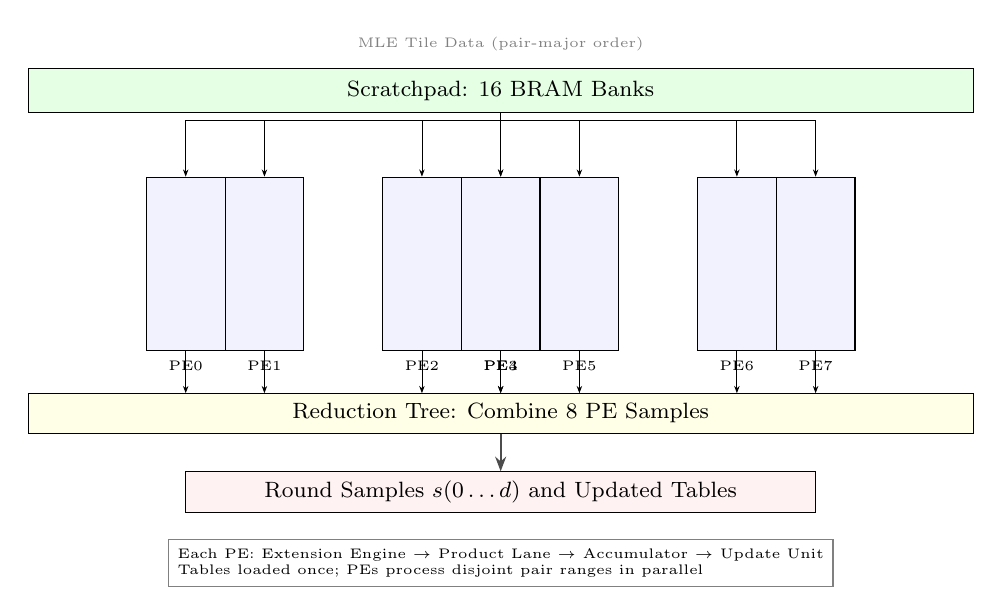
\begin{tikzpicture}[
    node distance=0.5cm and 0.3cm,
    spbox/.style={rectangle,draw=black,fill=green!10,minimum width=12cm,minimum height=0.55cm,font=\footnotesize},
    pebox/.style={rectangle,draw=black,fill=blue!5,minimum width=1.0cm,minimum height=2.2cm,font=\tiny},
    subbox/.style={rectangle,draw=black!50,fill=white,minimum width=0.85cm,minimum height=0.35cm,font=\tiny\sffamily},
    arr/.style={-{Stealth[scale=0.6]},line width=0.3pt},
    darr/.style={-{Stealth[scale=0.8]},line width=0.8pt,draw=black!70},
    lbl/.style={font=\tiny,text=black!50},
]

% Scratchpad
\node[spbox] (sp) at (0,2.5) {Scratchpad: 16 BRAM Banks};

% 8 PEs
\foreach \i in {0,1,2,3,4,5,6,7} {
    \pgfmathtruncatemacro{\x}{(\i-3.5)*1.3}
    \node[pebox,label=below:{\tiny PE\i}] (pe\i) at (\x, 0.3) {};
    \draw[arr] (sp.south) -- ++(0,-0.1) -| (pe\i.north);
}

% Reduction tree
\node[rectangle,draw=black,fill=yellow!10,minimum width=12cm,minimum height=0.5cm,font=\footnotesize] (red) at (0,-1.6) {Reduction Tree: Combine 8 PE Samples};
\foreach \i in {0,...,7} {
    \draw[arr] (pe\i.south) -- (pe\i.south |- red.north);
}

% Output
\node[rectangle,draw=black,fill=red!5,minimum width=8cm,minimum height=0.5cm,font=\footnotesize] (out) at (0,-2.6) {Round Samples $s(0\ldots d)$ and Updated Tables};
\draw[darr] (red.south) -- (out.north);

% Data flow labels
\node[lbl,above=0.1cm of sp] {MLE Tile Data (pair-major order)};

% Legend
\node[rectangle,draw=black!50,fill=white,minimum width=6cm,font=\tiny,align=left] (leg) at (0,-3.5) {
    Each PE: Extension Engine $\to$ Product Lane $\to$ Accumulator $\to$ Update Unit\\
    Tables loaded once; PEs process disjoint pair ranges in parallel
};

\end{tikzpicture}
\caption{Top-level accelerator architecture. Eight processing elements consume MLE table tiles from sixteen scratchpad banks. A reduction tree combines per-PE partial samples. The update unit writes halved MLE tables for the next round.}
\label{fig:architecture}
\end{figure}

\subsection{Multi-PE Orchestration}

The eight PEs process disjoint tile ranges in parallel. For a table of $N/2$ pairs, each PE receives $\lfloor N/(2N_{\mathrm{PE}})\rfloor$ pairs, with remainder pairs distributed across the first few PEs. When $N/2 < N_{\mathrm{PE}}$, the effective PE count is reduced to match the available parallelism. A reduction tree sums the per-PE round samples to produce the final $d+1$ output values. The MLE update is performed once at the top level, avoiding duplicate writes from multiple PEs.

Sixteen on-chip scratchpad banks---implemented via block RAM (BRAM)---supply MLE table data to the PEs. Each bank holds one tile of an MLE factor; the complete set of tables is loaded once at the start of computation via a \texttt{scratchpad\_load} function, then accessed by all PEs during the pair loop via \texttt{scratchpad\_read\_pair}. The banking scheme is organized such that PEs access disjoint banks per cycle, avoiding structural hazards.

\section{Implementation}

\subsection{HLS Design Flow}

The design is captured in synthesizable C++ using Vitis HLS 2023.2. All field elements are represented as \texttt{ap\_uint<256>}. The dual-interface design supports both standalone verification and deployment:

\begin{itemize}
\item \texttt{sumcheck\_round\_array}: BRAM interface with AXI-Lite control registers. Used for C-simulation and functional verification. Tables, samples, and updated tables are passed as multi-dimensional arrays with complete partitioning pragmas.
\item \texttt{sumcheck\_round\_axis}: AXI-Stream interface (planned) for DMA-based host communication, enabling integration into a PYNQ or embedded Linux overlay.
\end{itemize}

Compile-time parameters control the degree limit ($K_{\max}=6$), maximum table size ($N_{\max}=256$), number of PEs ($N_{\mathrm{PE}}=8$), and number of scratchpad banks ($N_{\mathrm{bank}}=16$). The IP catalog export targets the \texttt{xczu48dr-ffvg1517-2-e} device at a 200~MHz (5~ns) clock constraint.

\subsection{Verification Strategy}

A Python reference model computes expected values for all intermediate signals using deterministic test data. The model implements the affine evaluation rule, product-lane accumulation, and MLE update logic in exact agreement with the C++ implementation. Bit-exactness is enforced at the field-element granularity.

Seven test cases derived from the accelerator specification exercise distinct operational scenarios:

\begin{itemize}
\item \textbf{Case A} ($x_1 \cdot x_2 \cdot x_3$, round~1, challenges $r \in \{0,1,5\}$): Verifies the Extension Engine's affine interpolation. Expected samples: $[0,1,2,3]$.
\item \textbf{Case A chain} ($r_1=5, r_2=7, r_3=11$): Full three-round protocol chain collapsing to final scalar 385.
\item \textbf{Case B} ($x_1 \cdot x_2$ and $x_2 \cdot x_3$, round~1): Individual two-factor terms. Expected samples: $[1,1,1]$ and $[0,2,4]$.
\item \textbf{Case B combined}: Multi-term accumulation $x_1 \cdot x_2 + x_2 \cdot x_3$. Expected combined samples: $[1,3,5]$.
\end{itemize}

\section{Results}

\subsection{Synthesis}

Synthesis was performed for both a resource-constrained platform (PYNQ-Z2, \texttt{xc7z020}) and the target RFSoC~4x2 device (\texttt{xczu48dr}). Table~\ref{tab:synthesis} summarizes the post-synthesis resource utilization.

\begin{table}[t]
\centering
\caption{Post-synthesis resource utilization (8-PE configuration with scratchpad).}
\label{tab:synthesis}
\begin{tabular}{@{}lcccc@{}}
\toprule
\textbf{Resource} & \textbf{PYNQ-Z2} & \textbf{\%} & \textbf{RFSoC 4x2} & \textbf{\%} \\
\midrule
DSP slices  & 237  & 107.7\% & 466   & 10.9\% \\
BRAM tiles  & 60   & 21.4\%  & 154   & 7.1\%  \\
Flip-flops  & 66,984 & 62.9\% & 259,434 & 30.5\% \\
LUTs        & 21,221 & 39.9\% & 235,685 & 55.4\% \\
$F_{\max}$ & 140 MHz & ---   & 166 MHz & --- \\
\bottomrule
\end{tabular}
\end{table}

The PYNQ-Z2 implementation exceeds DSP availability (107.7\%), confirming that a reduced architecture or Montgomery-domain arithmetic is necessary for resource-constrained platforms. The RFSoC~4x2 implementation fits comfortably within all resource budgets. The estimated maximum clock frequency of 166~MHz approaches the 200~MHz target. LUT utilization at 55.4\% reflects the 8-way PE parallelism and complete array partitioning of the scratchpad banks, leaving substantial headroom for additional functionality.

\subsection{Scaling Analysis}

Scaling from one to eight PEs exhibits near-linear improvement in throughput, as the per-PE workload is independent and the scratchpad banking scheme avoids contention. The adaptive PE count mechanism gracefully degrades performance for small problem sizes where full parallelism cannot be exploited. The primary limitation on scaling is LUT utilization, driven by the complete array partitioning of the extension and product-lane buffers; relaxing the partitioning from ``complete'' to ``cyclic'' would reduce LUT usage at some cost to throughput.

\subsection{Architectural Parity with Reference Design}

The presented accelerator adheres to the zkPHIRE architecture described in~\cite{zkphire2026}. Specifically, it implements the PE microarchitecture (Extension Engine, Product Lane, Accumulator, Update Unit), the sixteen-scratchpad-bank buffering scheme, and the multi-PE tile-distribution strategy. The primary documented deviations are: (1)~regular-domain arithmetic using \texttt{ap\_uint} division rather than Montgomery multiplication; (2)~a maximum supported degree of $K_{\max}=6$ rather than the reference design's 31; and (3)~single-round SumCheck scope rather than the full HyperPlonk protocol stack (ZeroCheck, PermCheck, OpenCheck).

\section{Conclusion}

This work has presented a programmable, FPGA-based accelerator for one round of the SumCheck protocol operating over the BN254 scalar field. The architecture employs eight parallel processing elements, sixteen scratchpad buffer banks, and an adaptive PE dispatch mechanism. C-simulation verification confirms bit-exact agreement with a Python golden model across seven deterministic test cases. Synthesis results on the Xilinx RFSoC~4x2 demonstrate feasible resource utilization with substantial headroom for integration into a complete ZKP prover pipeline.

Future work includes: (1)~implementing Montgomery modular multiplication to reduce DSP utilization; (2)~extending the maximum supported degree to 31; (3)~integrating the accelerator into a full HyperPlonk protocol stack with ZeroCheck, PermCheck, and OpenCheck support; and (4)~deploying the combined system on an RFSoC platform for end-to-end prover benchmarking.

\bibliographystyle{IEEEtran}
\begin{thebibliography}{1}

\bibitem{lund1992algebraic}
C.~Lund, L.~Fortnow, H.~Karloff, and N.~Nisan,
``Algebraic methods for interactive proof systems,''
\textit{Journal of the ACM}, vol.~39, no.~4, pp.~859--868, 1992.

\bibitem{chen2022hyperplonk}
B.~Chen, B.~B{\"u}nz, D.~Boneh, and Z.~Zhang,
``HyperPlonk: Plonk with linear-time prover and high-degree custom gates,''
in \textit{Advances in Cryptology---EUROCRYPT 2022}, 2022.

\bibitem{setty2020spartan}
S.~Setty,
``Spartan: Efficient and general-purpose zkSNARKs without trusted setup,''
in \textit{Advances in Cryptology---CRYPTO 2020}, 2020.

\bibitem{gabizon2019plonk}
A.~Gabizon, Z.~J.~Williamson, and O.~Ciobotaru,
``PLONK: Permutations over Lagrange-bases for oecumenical noninteractive arguments of knowledge,''
Cryptology ePrint Archive, Report 2019/953, 2019.

\bibitem{montgomery1985modular}
P.~L.~Montgomery,
``Modular multiplication without trial division,''
\textit{Mathematics of Computation}, vol.~44, no.~170, pp.~519--521, 1985.

\bibitem{zkphire2026}
A.~Daftardar, J.~Mo, J.~Ah-kiow, B.~B{\"u}nz, S.~Garg, and B.~Reagen,
``zkPHIRE: A Programmable Accelerator for ZKPs over HIgh-degRee, Expressive Gates,''
in \textit{Proc. HPCA}, 2026.

\end{thebibliography}

\end{document}
